%第4章:実験結果・考察
本章ではV字開発モデルにおけるて実装及び検証について述べる。ここでは具体的な実装方法について述べる。
\section{実装・実験環境}
実装はグループで行い、エッジ処理側は真鍋樹が行った。この章では筆者が担当した、サーバ側の実装についてのみ述べる。ここでは、エッジ処理側のことをクライアントと呼ぶ。実装に使用したプログラム言語は、クライアント、サーバのどちらもPython3である。


\subsection*{実験環境}
実験環境で使用したハードウェアのスペックを以下の表\ref{spec}に示す。
\begin{table}[htb]
\begin{center}
\caption{実行環境}
\begin{tabular}{|c|c|c|c|c|} \hline
処理担当 & OS & CPU & RAM & GPU \\ \hline
サーバ側 & Windows10 64bit Pro & Core2Duo E7500 2.93GHz & 4GB & GT740 \\ \hline
エッジ側 & RaspberryPi 3B(Rasbian) & Broadcom 1.2GHz & 1GB & None \\ \hline
\end{tabular}
\label{spec}
	\end{center}
\end{table}


実験環境で使用したライブラリ、プログラム言語を以下の表\ref{library_spec}に示す。
\begin{table}[htb]
\begin{center}
\caption{使用ライブラリ・使用言語}
\begin{tabular}{|c|c|c|c|c|} \hline
処理担当 & ライブラリ・使用言語名 & バージョン & 使用目的 \\ \hline \hline
サーバ側 & Python3 & 3.7.4 & メイン処理	\\ \hline
サーバ側 & OpenCV & 4.1.2 & 画像切り取り\\ \hline
サーバ側 & Yolo & 3 & バーコード領域取得\\ \hline
サーバ側 & CUDA & 10.1 & 学習に使用\\ \hline
サーバ側 & pyzbar & 0.1.8 & バーコード番号取得\\ \hline
サーバ側 & mysqlclient & 1.4.6 & DB操作\\ \hline \hline
Webページ & XAMPP & 3.2.4 & Webページ、DBホスト\\ \hline
Webページ & apache2 & 2.4.41 & Webページホスト\\ \hline
Webページ & MariaDB & 10.4.10 & DB\\ \hline
Webページ & PHP & 7.3.12 & Webページ処理、DB操作\\ \hline \hline
エッジ側 & Python3 & 3.7.3 & メイン処理		\\ \hline
エッジ側 & OpenCV & 3.4.3 & Webカメラ操作\\ \hline
\end{tabular}
\label{library_spec}
	\end{center}
\end{table}


\newpage

\subsection*{サーバ通信}
クライアントとのデータのやり取りを含めた連携には、通信処理が必要不可欠になる。クライアントは、距離センサの反応後、カメラを起動し複数の画像を撮影する。クライアントからサーバへ送信するデータは、画像データとフラグをセットしたものである。しかしながら、ソケット通信において送信処理が複数回であったとしても、受信処理ではひとまとまりのデータとして受け取られることがある。その問題を防ぐために、送信データのヘッダにデータのサイズを書き込む手段をとった。
クライアントから送られてきた画像データはバイナリ形式になっているので、OpenCV\cite{opencv}のフォーマットに変換する。

\subsection*{Yoloによるバーコード領域特定}
Yoloを使用した理由は、pyzbar\cite{pyzbar}の識別精度にある問題があったからである。pyzbar\cite{pyzbar}は、近距離で撮影したバーコードの画像の認識はできるが、距離が離れると識別しなくなる。これは、画像の中に占めるバーコード部分が少なくなることが原因であると考えられる。そこで、Yoloを使用し画像からバーコードの部分の座標を取得する。画像のうち、バーコードの部分のみをpyzbarに渡すことで、距離が離れていても近距離で撮影したのと同じ効果が得られるようになった。学習には、バーコードの画像を約2000枚用意した。Yoloの実行はサーバ側で行う。当初、クライアント側であるRaspberryPiでYoloを実行すればサーバは不要になり、通信におけるタイムラグもなくなることが仮定された。ところが、RaspberryPiの性能ではYoloを、高い識別精度を保ったままリアルタイムに動作させることは、性能上難しいと判断したためサーバで行うことになった。

\newpage

\subsection*{DBを使用した商品情報の管理}
カゴの中の商品の管理と、商品自体の情報の管理のために、DBを使用した。本研究ではMariaDBを使用した。カゴDBの構造を以下に示す。
始めに、商品自体のデータを管理するitemテーブルを表\ref{item_db}に示す。janとはJANコードのことであり、スマートモビリティレジ番号である。titleは、商品名のことである。priceは、商品の価格を示す。
image\_urlは、商品の画像があるURLを示している。最後の、image\_rawはこのシステムでは使用していないが、画像データそのものを格納する。
\begin{table}[htbp]
\centering
\caption{itemテーブル}
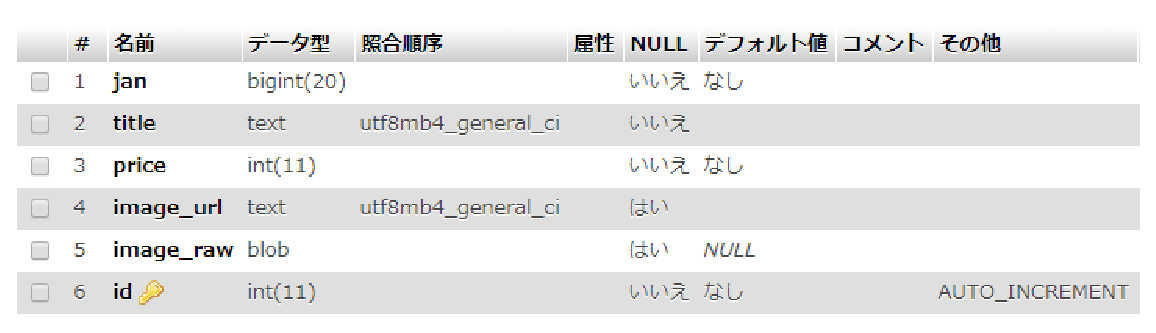
\includegraphics[width=15cm]{./pic/item_db.eps}
\label{item_db}
\end{table}

\newpage

次に、cartテーブルの構造を表\ref{cart_db}に示す。idは、テーブルのレコードの固有番号を示すためにある。janは、JANコードのことである。cart\_idはカートの固有番号を示す。この番号でカートごとの区別を行う。この番号があることで複数カートを運用した際も区別することができる。
%%%商品DB
\begin{table}[htbp]
\centering
\caption{cartテーブル}
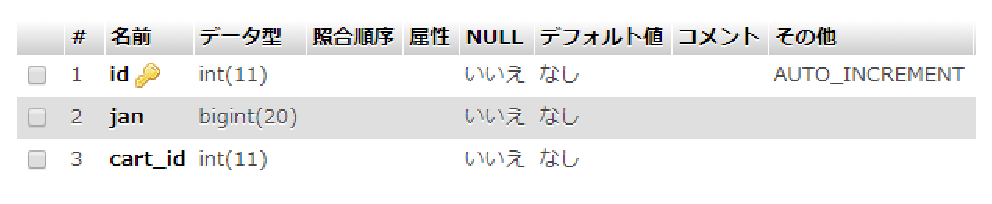
\includegraphics[width=15cm]{./pic/cart_db.eps}
\label{cart_db}
\end{table}


customerテーブルの構造を表\ref{customer_db}に示す。このcustomerテーブルは、顧客情報を管理する。idは顧客の固有番号を示す。balanceは、顧客の所持金額を示す。

\begin{table}[htbp]
\centering
\caption{customerテーブル}
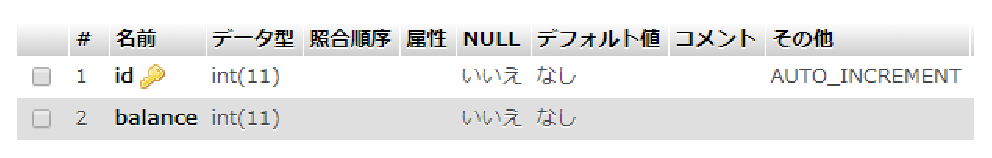
\includegraphics[width=15cm]{./pic/customer.eps}
\label{customer_db}
\end{table}

\newpage

\subsection*{決済システム}
設計段階では、決済システムの動作は、ユーザが退店する際に自動で行われる。しかし、その機能を実装するには時間の都合上難しいと判断したため、仮の決済用のWebページを作成してテストを行っている。Webページ作成にはPHPとHtmlを使用した。以下にWebページの動作の手順を示す。

\subsection*{カート画面}
以下の図\ref{web_cart}は、どのカートを使用するか選択するためにある。
\begin{figure}[htbp]
\centering
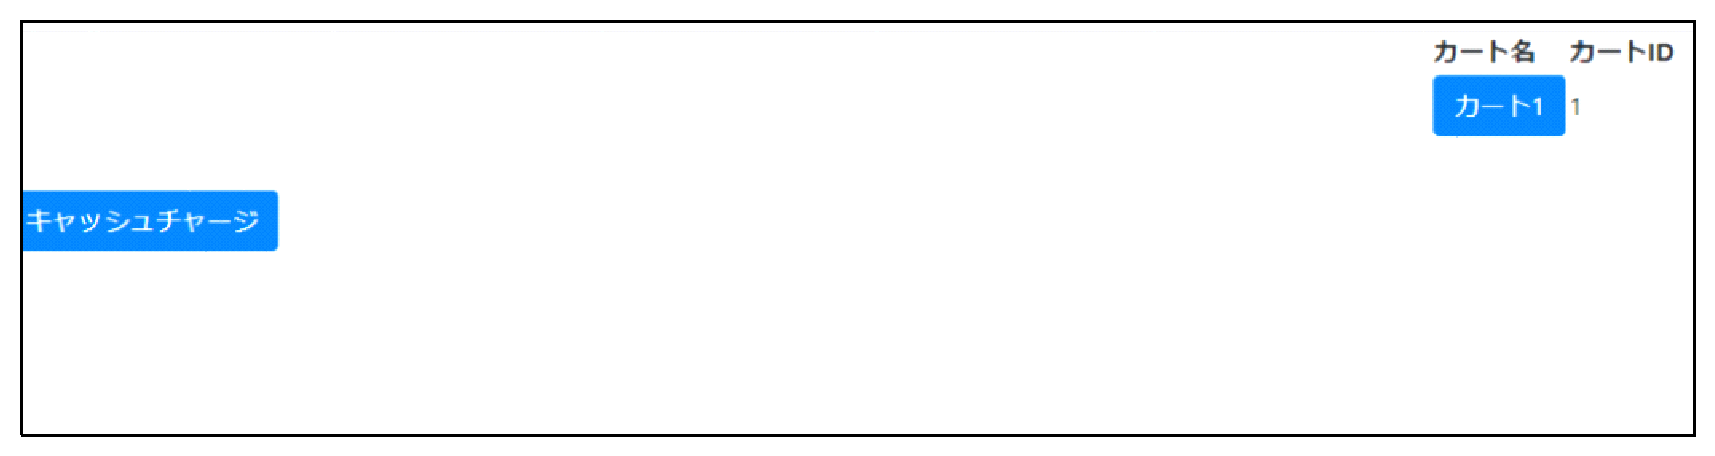
\includegraphics[width=15cm]{./pic/web/1.eps}
\caption{Webページ カート画面}
\label{web_cart}
\end{figure}

\subsection*{カート内商品一覧}
図\ref{web_cart_items}は、カート内にある購入予定商品の一覧を表している。表示内容は、商品名と価格、商品画像、個数の4つである。ページ内にある緑のボタンを押すと、会計が行われる。
\begin{figure}[htbp]
\centering
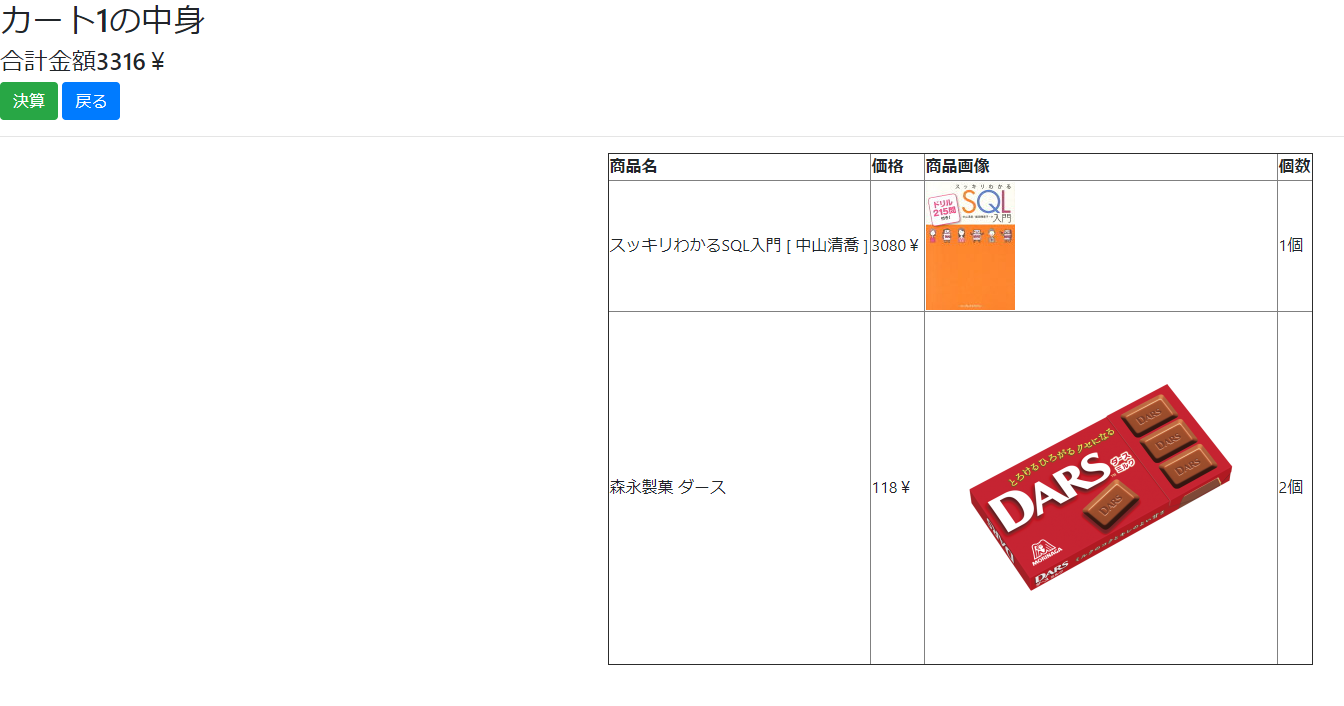
\includegraphics[width=15cm]{./pic/web/2.eps}
\caption{Webページ カート内商品一覧}
\label{web_cart_items}
\end{figure}

\subsection*{決済完了画面}
図\ref{web_cart_items}のページで緑のボタンを押すと、図\ref{web_checksum}画面に移行する。移行後は図\ref{web_checksum}のとおりに顧客の所持金から購入金額が差し引かれ、残高が表示される。また、所持金が購入金額が下回っていた場合は、所持金額が足りないと警告され決済は行われない。
\begin{figure}[htbp]
\centering
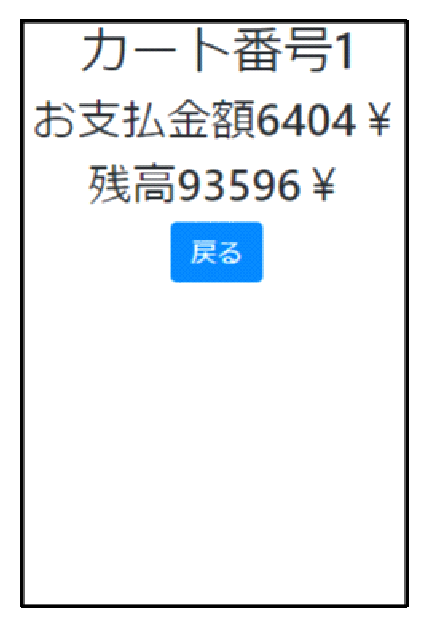
\includegraphics[width=10cm,height=10cm]{./pic/web/3.eps}
\caption{Webページ 決済完了}
\label{web_checksum}
\end{figure}

\newpage